\documentclass{article}

\usepackage{graphicx}
\usepackage{tikz}
\usepackage{tikzsymbols}
\usetikzlibrary{calc,patterns,shapes.geometric}
\pagestyle{empty}
\usepackage[margin=0pt]{geometry}
\geometry{papersize={14in,12in}}

\def\centerarc[#1](#2)(#3:#4:#5){\draw[#1] ($(#2)+({#5*cos(#3)},{#5*sin(#3)})$) arc (#3:#4:#5);}

\begin{document}
	\begin{figure}
		\centering
		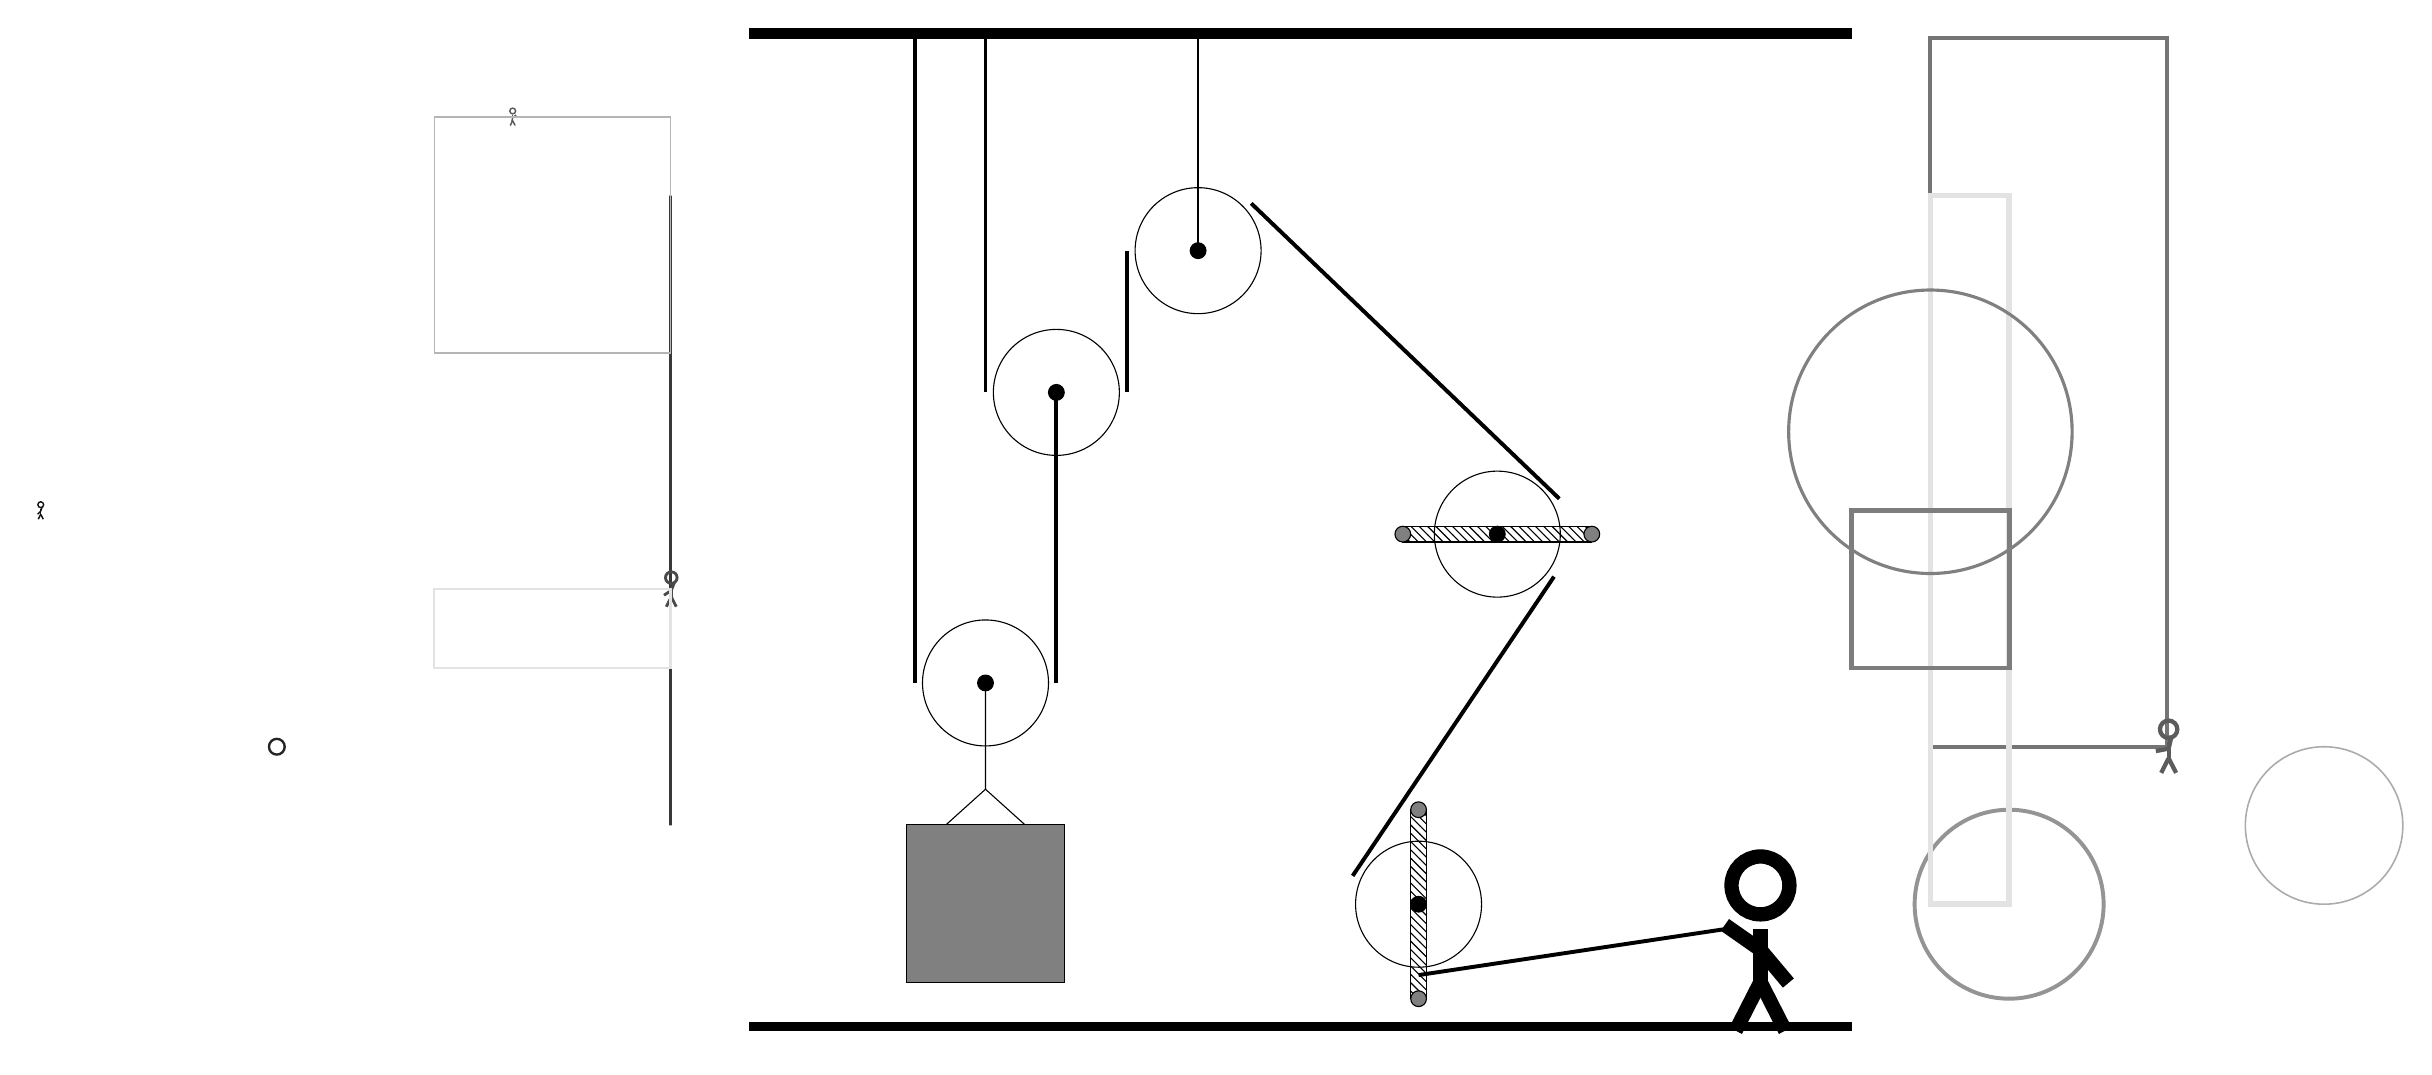
\begin{tikzpicture}
			%%%%% START %%%%%
			
			\draw[fill=black] (-2, 9) rectangle (12, 9.125);
			
			\draw (1, 0.81) circle (0.8);
			\draw[fill=black] (1, 0.81) circle (0.1);
			
			\draw (1.9, 4.5) circle (0.8);
			\draw[fill=black] (1.9, 4.5) circle (0.1);
			
			\draw (3.7, 6.3) circle (0.8);
			\draw[fill=black] (3.7, 6.3) circle (0.1);
			\draw[thick] (3.7, 6.3) -- (3.7, 9);
			
			\draw (6.5, -2) circle (0.8);
			\draw[fill=black] (6.5, -2) circle (0.1);
			\draw[pattern=north west lines, pattern color=black] (6.4, -0.8) rectangle (6.6, -3.2);
			\draw[fill=black!50] (6.5, -0.8) circle (0.1);
			\draw[fill=black!50] (6.5, -3.2) circle (0.1);
			
			\draw (7.5, 2.7) circle (0.8);
			\draw[fill=black] (7.5, 2.7) circle (0.1);
			\draw[pattern=north west lines, pattern color=black] (6.3, 2.8) rectangle (8.7, 2.6);
			\draw[fill=black!50] (6.3, 2.7) circle (0.1);
			\draw[fill=black!50] (8.7, 2.7) circle (0.1);
			
			\draw (1, 0.81) -- (1, -0.54) -- (0.5, -0.99) -- (1.5, -0.99) -- (1, -0.54);
			\draw[fill=black!50] (0, -0.99) rectangle (2, -2.99);
			
			\draw[line width=0.3mm, color=black!78] (-3, -1) rectangle (-3, 7);
			
			\draw [line width=0.5mm, color=black!42](14, -2) circle (1.2);
			\node[line width=0.5mm, color=black!65] at (-5, 8) {\Strichmaxerl[1][78][34]};
			\draw [line width=0.2mm, color=black!33](18, -1) circle (1.0);
			\draw[line width=0.5mm, color=black!54] (13, 9) rectangle (16, 0);
			
			\draw[line width=0.2mm, color=black!29] (-3, 5) rectangle (-6, 8);
			
			\draw[line width=0.7mm, color=black!11] (14, 7) rectangle (13, -2);
			
			\node[line width=0.3mm, color=black!71] at (-3, 2) {\Strichmaxerl[2][33][69]};
			\draw[line width=0.3mm, color=black!11] (-3, 2) rectangle (-6, 1);
			\draw[line width=0.6mm, color=black!51] (14, 3) rectangle (12, 1);
			\node[line width=0.7mm, color=black!93] at (-11, 3) {\Strichmaxerl[1][44][71]};
			\draw [line width=0.3mm, color=black!86](-8, 0) circle (0.1);
			\draw [line width=0.4mm, color=black!50](13, 4) circle (1.8);
			
			\node[line width=0.7mm, color=black!64] at (16, 0) {\Strichmaxerl[3][11][77]};
			
			\draw[line width=0.5mm] (0.1, 9) -- (0.1, 0.81);
			\centerarc[line width=0.5mm](1, 0.81)(180:360:0.9);
			\draw[line width=0.5mm](1.9, 0.81) -- (1.9, 4.5);
			\draw[line width=0.5mm] (1.0, 9) -- (1.0, 4.5);
			\centerarc[line width=0.5mm](1.9, 4.5)(180:360:0.9);
			\draw[line width=0.5mm](2.8, 4.5) -- (2.8, 6.3);
			\centerarc[line width=0.5mm](3.7, 6.3)(35:180:0.9);
			\draw[line width=0.5mm] (4.375, 6.9) -- (8.2875, 3.15);
			\centerarc[line width=0.5mm](7.5, 2.7)(215:135:-0.9);
			\draw[line width=0.5mm](8.22, 2.16) -- (5.663, -1.64);
			\centerarc[line width=0.5mm](6.5, -2)(-30:100:-0.9);
			\draw[line width=0.5mm](6.5, -2.9) -- (10.5, -2.3);
			
			\node at (10.8, -2.5) {\Strichmaxerl[10][-35][-50]};
			
			\draw[fill=black] (-2, -3.5) rectangle (12, -3.6);
			
			%%%%% END %%%%%
		\end{tikzpicture}
	\end{figure}	
\end{document}